% ---------------------------------------------------------------------------
% Supplementary appendix for the RECOMB 2027 submission.
%
% RECOMB accepts one supplementary PDF of unlimited length, which reviewers
% may or may not read. Everything here supports a claim made in the main text;
% nothing here is needed to follow it.
%
% Build:  pdflatex appendix && bibtex appendix && pdflatex appendix x2
% ---------------------------------------------------------------------------
\documentclass[10pt]{article}

\usepackage[utf8]{inputenc}
\usepackage[T1]{fontenc}
\usepackage[margin=1in]{geometry}
\usepackage{graphicx}
\usepackage{booktabs}
\usepackage{amsmath,amssymb}
\usepackage[expansion=false]{microtype}
\usepackage[labelfont=bf,font=small]{caption}
\usepackage[numbers,sort&compress]{natbib}
\usepackage[hidelinks]{hyperref}
\usepackage{verbatim}
\usepackage{fancyvrb}

\graphicspath{{../figures/}}
\renewcommand{\thesection}{S\arabic{section}}
\renewcommand{\thefigure}{S\arabic{figure}}
\renewcommand{\thetable}{S\arabic{table}}

\title{\textbf{Supplementary appendix}\\[2pt]
\large Factor-combination discovery is stochastic threshold group testing:
a counterfactual replay of the 2006 reprogramming screen}
\author{Mashal Saleh Alkhalifah}
\date{\today}

\begin{document}
\maketitle

\noindent
This appendix carries the campaigns behind the intervals and paired tests in
the main text, the figures the page limit displaced, and the complete
statistical report as the analysis code emits it. Every number in the main
text can be traced to a section here, and every section here can be
regenerated from the public repository
(\url{https://github.com/mashal-alkhalifah/yamanaka-replay}) without rerunning
any simulation: the per-run CSVs are committed, and
\texttt{analysis/analyze.py} reads them.

\tableofcontents

% ===========================================================================
\section{The experimental campaign}

\begin{table}[h]
  \centering
  \small
  \begin{tabular}{llr l}
    \toprule
    Script & What it varies & Runs & Supports \\
    \midrule
    \texttt{01\_main\_comparison} & the four strategies, small & 80 & demonstration \\
    \texttt{02\_prior\_robustness} & prior quality, small & 60 & demonstration \\
    \texttt{03\_misspecification} & one assumption at a time & 120 & S2 \\
    \texttt{04\_trace\_single\_run} & one run, experiment by experiment & 1 & demonstration \\
    \texttt{05\_scale\_main} & the four strategies, paired & 1{,}200 & main text \S3.1 \\
    \texttt{06\_synergy\_threshold} & true vs assumed synergy & 1{,}100 & S2 \\
    \texttt{07\_stopping\_rule} & stopping threshold & 1{,}680 & S3 \\
    \texttt{08\_scaling} & 24 to 60 candidates & 300 & main text \S3.2 \\
    \texttt{09\_prior\_quality} & strength $\times$ coverage $\times$ breadth & 1{,}800 & S4 \\
    \texttt{10\_unknown\_cardinality} & fixed vs latent recipe size & 240 & main text \S3.3 \\
    \texttt{11\_classical\_baseline} & half-removal across sizes & 270 & main text \S3.2 \\
    \texttt{12\_cardinality\_baselines} & two-stage and model-free & 225 & main text \S3.3 \\
    \texttt{13\_measured\_gap} & $\rho$ drawn from measurement & 2{,}200 & main text \S3.4 \\
    \texttt{14\_norman\_retrospective} & measured queries only & 120 & main text \S3.6 \\
    \texttt{15\_proposal\_ablation} & only the proposal set & 184 & main text \S3.2 \\
    \texttt{16\_latent\_gap} & inferring $\rho$ vs a pilot & 1{,}500 & main text \S3.5 \\
    \bottomrule
  \end{tabular}
  \caption{Every campaign, with the claim it supports. Runs are independent
  replicates recorded individually, so all aggregation is reproducible without
  re-simulation. Strategies within an experiment share hidden recipes and noise
  seeds, making every comparison paired.}
  \label{tab:campaigns}
\end{table}

Reference environment: Linux 6.18, x86\_64, 2 cores, 7.8\,GB RAM, Python
3.13.16, NumPy 2.5.3. No GPU and no network access are required. The
statistics layer is implemented directly in NumPy to hold the dependency list
at one package, and is therefore tested: \texttt{analysis/test\_stats.py}
checks each estimator against a closed-form or planted-truth answer, including
the permutation test's false-positive rate under the null.

\paragraph{Three corrections this campaign forced on its own earlier claims.}
An earlier version of this work reported that absent graded synergy was a
structural failure, that the design step was independent of hypothesis-space
size, and that the adaptive designer's advantage ended at 48 candidates.
Experiment 6 refuted the first (Section~\ref{sec:s-synergy}), experiment 8
refuted the second, and experiment 15 refuted the third (main text \S3.2).
They are recorded here rather than quietly dropped, because a reader deciding
how much to trust the remaining claims should know how the earlier ones fared.

% ===========================================================================
\section{Model error: absent signal versus wrong signal}
\label{sec:s-synergy}

\begin{figure}[tbp]
  \centering
  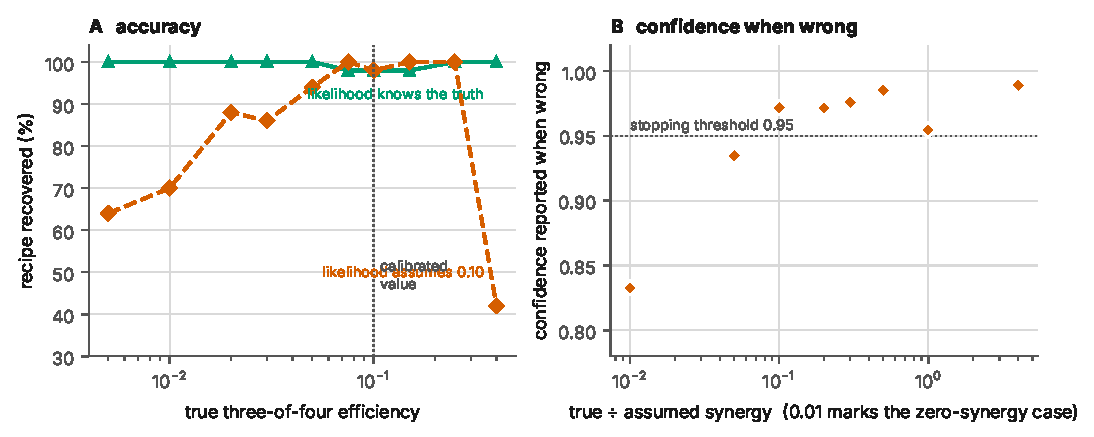
\includegraphics[width=\textwidth]{fig3_calibration.pdf}
  \caption{\textbf{True three-of-four efficiency against what the searcher
  assumes.} Arms are paired by run, so only the searcher's assumption differs.
  A searcher told the truth succeeds at every true value tested, including
  zero; a searcher holding the calibrated 0.10 degrades asymmetrically, and
  degrades worst when it \emph{over}-estimates the partial effect.}
  \label{fig:calibration}
\end{figure}

Making the oracle disagree with the designer one assumption at a time
(experiment 3) suggested that removing graded synergy was fatal: 43\% success.
That experiment conflated two things, removing the partial signal from the
assay while leaving the searcher believing in it. Experiment 6 separates them.
With no graded synergy whatsoever and a searcher that knows it, the method
succeeds in 100\% of runs at a median of 22 experiments: it degenerates into
pure group testing, pays 2.2$\times$ for the lost gradient, and is still 64\%
cheaper than the 2006 protocol. The earlier figure was misspecification, not
lost information.

What does matter is how wrong the assumed value is and in which direction, and
the window is asymmetric. Under-estimating the partial effect fivefold still
succeeds in 70\% of runs; over-estimating it fourfold drops to 42\%, and
reports a confidence of 0.989 while doing so. This asymmetry is what makes the
measured audit in the main text consequential: the calibrated 0.10 sits on the
dangerous side of the true value, not the safe one.

% ===========================================================================
\section{The stopping rule}
\label{sec:s-stopping}

\begin{figure}[tbp]
  \centering
  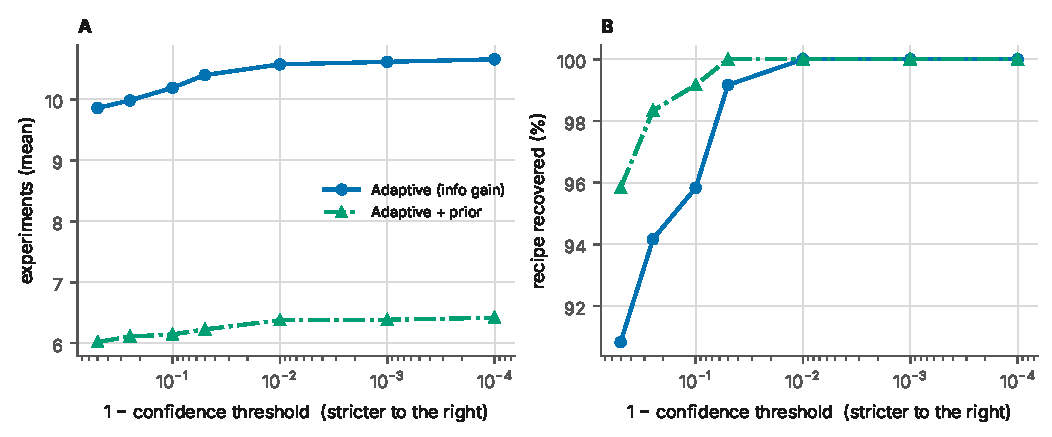
\includegraphics[width=\textwidth]{fig5_stopping_rule.pdf}
  \caption{\textbf{Cost and reliability against the stopping threshold.} The
  rule is nearly free over the usable range, and the posterior is well
  calibrated \emph{when the model is right} --- which is the condition the main
  text's \S3.4 removes.}
  \label{fig:stopping}
\end{figure}

Raising the stopping threshold from 0.50 to 0.99 costs little and buys
reliability, so the rule is not a tuning knob the results depend on. Under a
correctly specified model the reported confidence tracks the realised success
rate closely. That calibration is conditional on the model, and the main text
shows what happens when it is not: the same rule returns 0.991 on runs that
end wrong. A stopping rule can only be as honest as the likelihood behind it.

% ===========================================================================
\section{Prior quality}
\label{sec:s-prior}

A literature prior up-weighting eight factors reduces the median from 10 to 6
experiments. Experiment 9 varies its quality along three axes --- strength,
coverage (how many true factors it includes) and breadth (how many decoys) ---
over 1{,}800 runs. The prior degrades gracefully: a factor the literature
missed still carries non-zero mass and can be recovered from data, so the
method does not fail when the prior is wrong, it merely stops helping. The one
reading to avoid is treating the prior's benefit as scale-free. In experiment
8 the informed arm appears flat in $n$ only because prior quality is held
constant, up-weighting eight factors regardless of list length; a longer
candidate list in practice implies a less informative prior, so that curve is
an upper bound conditional on prior quality, not a prediction.

% ===========================================================================
\section{Scaling, the classical baseline, and the proposal generator}
\label{sec:s-scaling}

\begin{figure}[tbp]
  \centering
  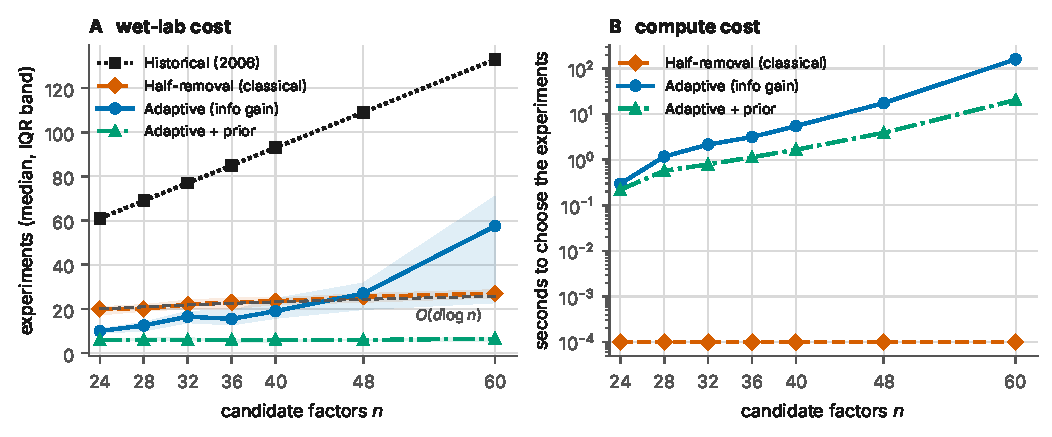
\includegraphics[width=\textwidth]{fig2_scaling.pdf}
  \caption{\textbf{Growth with candidate-list size, as first measured.}
  (A) Wet-lab cost, medians with interquartile bands, against the
  $O(d \log n)$ reference curve scaled at the smallest list. (B) Compute spent
  choosing experiments. This is the measurement that produced the regime claim
  the main text then withdraws.}
  \label{fig:scaling}
\end{figure}

\begin{figure}[tbp]
  \centering
  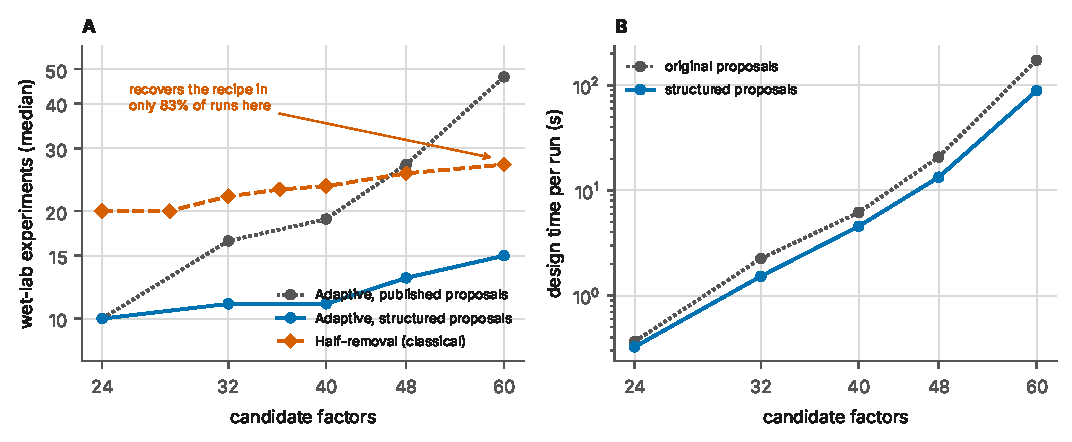
\includegraphics[width=\textwidth]{fig9_proposals.pdf}
  \caption{\textbf{Changing only which pools may be scored.} (A) Median
  wet-lab cost against candidate-list size for the published generator, the
  structured one, and half-removal. Scoring rule, posterior, oracle, recipes,
  seeds and the number of pools scored per round are identical across the two
  adaptive curves. (B) The design-time price of the change, which is negative:
  the structured proposals need fewer rounds than their larger pools cost.}
  \label{fig:proposals}
\end{figure}

Compute cost grows as roughly $H^{1.5}$ in the hypothesis count $H$. The
correct narrow claim is that the design step is independent of \emph{how
concentrated the posterior is} --- the $k+1$ overlap-class collapse is real ---
but it remains linear in the \emph{size of the enumerated space}, and the
number of rounds grows too. Exact enumeration is the binding constraint past
about 60 candidates, and the structured proposals of the main text do not
change this; they change only the number of wet-lab experiments.

The structured generator is also faster in wall-clock terms despite proposing
larger pools, because it needs fewer rounds: 89\,s per run at 60 candidates
against 173\,s. Part of that is a separate exact optimisation, counting
overlaps over whichever side of the pool is smaller, verified against the
direct computation on 400 random pools at two candidate counts.

% ===========================================================================
\section{The measured audit in full}
\label{sec:s-real}

\begin{figure}[tbp]
  \centering
  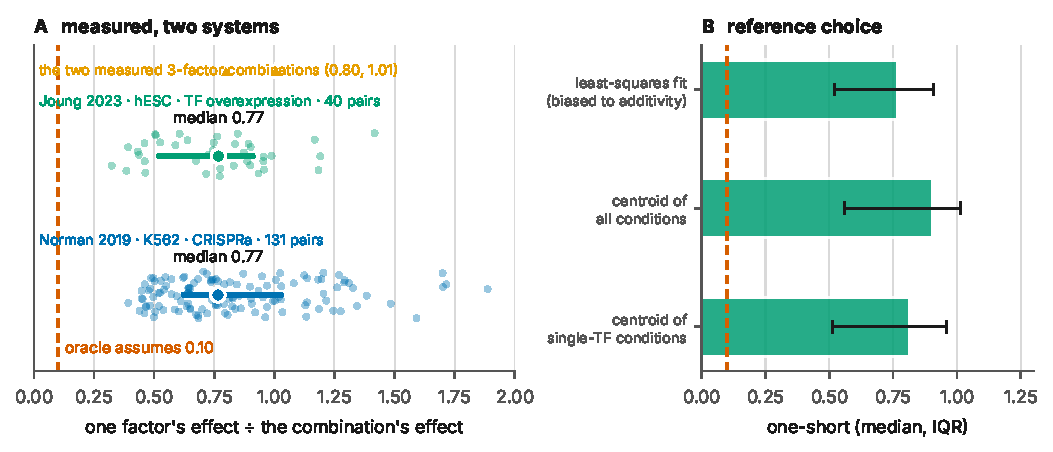
\includegraphics[width=\textwidth]{fig6_real_data.pdf}
  \caption{\textbf{What one factor of a measured combination reproduces.}
  (A) The one-short ratio for 131 gene pairs in K562 \citep{norman2019} and 40
  transcription-factor pairs in human embryonic stem cells
  \citep{joung2023}, with the two measured three-factor combinations marked.
  (B) The hESC subset has no unperturbed control, so three references are
  reported; the conclusion holds under all three.}
  \label{fig:real}
\end{figure}

Two observations beyond the headline median. First, departures from additivity
are common but modest: in Norman the median ratio of a pair's effect to the
sum of its singles is 0.91, with 47\% sub-additive and 27\% super-additive, and
only 28\% of pairs have an additivity residual exceeding their own sampling
noise, estimated by regressing squared residuals on
$1/n_{AB} + 1/n_A + 1/n_B$. Second, the two systems differ in \emph{where} the
interaction lives: the median $R^2$ of a pair on its two singles is 0.86 in
K562 but 0.64 in hESCs, so combinations in the stem-cell system leave the
plane spanned by their constituents more while their magnitudes stay
near-additive.

The result is not an artefact of measuring effect size by a Euclidean norm.
Repeating the Norman analysis with threshold-like functionals --- the number of
genes moving more than 0.25 or 0.5 in log space --- lowers the median to 0.48
and 0.50 and raises the fraction below 0.20 to 25\% and 22\%, but no functional
produces a median near 0.10.

% ===========================================================================
\clearpage
\section{Complete statistical report}
\label{sec:s-report}

What follows is the verbatim output of \texttt{analysis/analyze.py}, which
reads the committed per-run CSVs and runs no simulation. Box-drawing
characters have been transliterated to ASCII for typesetting; the file itself
is in the repository at \texttt{results/analysis\_report.txt}.

\VerbatimInput[fontsize=\tiny, numbers=none, frame=none]{analysis_report_ascii.txt}

\bibliographystyle{unsrtnat}
\bibliography{refs}

\end{document}
